\documentclass{article}

\usepackage{amsmath}
\usepackage{amsfonts}
\usepackage{multicol}
\usepackage[document]{ragged2e}

\begin{document}

\title{Ambiguously-Typed Lambda Calculus}

\author{Athan Clark}

\date{}

\maketitle

\begin{abstract}
\begin{flushleft}
Here, we present the ambiguously-typed lambda calculus - a size-dependent type
system measuring the \textit{shape} of terms, based on their context, and an
additional \textit{substitution system}, facilitating the merge and sort of
multiple terms' parameters.
\end{flushleft}
\end{abstract}

\cite{Author2year2}

%-------------------------------------------------%
\section{Motivation}
%-------------------------------------------------%

The Simply-Typed Lambda Calculus follows from the untyped lambda calculus in that
there is structural assignment to parameters, and each "step" of arity is
mechanically separated with $\rightarrow$. Values are given type labels, and
arguments' types are checked one-for-one to the specification signature. Higher
order function application, the true nature of lambda calculus, is retained
through parameter specification (or type signature) nesting. The grammars are
structured as follows:

\center{
\begin{multicols}{2}
\begin{minipage}{\columnwidth}
\center{
\underline{Untyped Lambda Calculus}
\vspace{11mm}
\begin{align*}
e = \hspace{2mm} & x\\
                 & \lambda x.e\\
                 & e \hspace{2mm} e
\end{align*}
}
\end{minipage}
\break
\begin{minipage}{\columnwidth}
\center{
\underline{Simply-Typed Lambda Calculus}
\begin{align*}
\tau ::= \tau \rightarrow \tau | T \textrm{\hspace{2mm} where \hspace{2mm}} T \in B
\end{align*}
\begin{align*}
e = \hspace{2mm} & x : \tau\\
                 & \lambda (x : \tau).e\\
                 & e \hspace{2mm} e\\
                 & c
\end{align*}
}
\end{minipage}
\end{multicols}
}

\begin{flushleft}
$c$ is a "term constant", such that $c$ is an inhabitant of a type $T$ included
in our working set $B$.\\
\break
The untyped lambda calculus gives us a foundation to base all others off of -
it is the minimum embodyment of higher-order function application and abstraction.
But, there is no beginning, and no end; it suffices only to provide action, and
not results. This is what the simply-typed lambda calculus fills - it provides
an encoding of the finite "end" of an expression in it's type, by utilizing
$\rightarrow$ for each step.

The simply-typed lambda calculus makes a critical decision - it gives up
infinite arity for the sake of traction and decidable termination.
We present the ambiguously-typing scheme to give back our
infinite arity, at the cost of detailed knowledge.
\end{flushleft}

%-------------------------------------------------%
\section{Overview}
%-------------------------------------------------%

\begin{flushleft}
Our system encodes arity in the space of variables quantified over natural
numbers, and constrained based on requirements induced by application and
abstraction context. This is a size-dependent type system variant, similar to
Cryptol. Indeed, our "size" of terms is ambiguous - it gives us no insight
to how parameters are resolved. We additionally include a \textit{parameter
resulution system} - a method for unifying substitutions. We later shoe-horn
a pseudo-monoid instance to our system, with the \textit{union} of lambdas as our
monoidal append.

Our type system also has decidable and total type inference; the size-dependent
system initially assumes all terms to be polymorphic in arity, then, depending
on how terms are used, minimum bounds are enforced in our sizes based on natural
number literals.
\end{flushleft}

\subsection{Brief Example}

\begin{align}
x &: \forall a \in \mathbb{N}. \Rightarrow &a\label{ex1:eq1}\\
f &: \forall b \in \mathbb{N}. \Rightarrow &b\label{ex1:eq2}\\
f \, x &: \forall a \in \mathbb{N}, b \in \mathbb{N}.
\{a \geq 1\} \Rightarrow &(a - 1) + b\label{ex1:eq3}\\
\end{align}

\begin{flushleft}
In our first examples \ref{ex1:eq1} and \ref{ex1:eq2}, their sizes are purely
polymorphic because there is no context telling us how the expression should
behave. In \ref{ex1:eq3}, we can see some interesting ideas: because $f$ was
applied to $x$, we now have a constraint bound to it's
type variable\footnote{A degenerate consequence of our structureless arity specification
is that a type variable's reference to it's term must be syntactically in-order -
$\forall \, a \, b$ over $x \, y$ will match $x$ with $a$, and $y$ with $b$.}.
Also, because $x$ consumed one parameter in $a$, we must decrement it. Lastly,
we take the left-over parameters in $x$ and $a-1$ and combine them; in our
(commutative) sized interpretation, this is simply addition\footnote{This
neglects the order that the parameters get combined intentionally.}.

Note that I didn't include the type of a lambda. Please be patient; we will find
that a function's size depends on it's body.
\end{flushleft}

\subsection{Hand-Wave}

Here is the grammar:

\begin{align}
e = \hspace{2mm} & x           & \mathrm{term}\\
                 & \lambda x.e & \mathrm{abstraction}\\
                 & \lceil e \hspace{2mm} e & \mathrm{inner \, application}\\
                 & e \hspace{2mm} \lceil e & \mathrm{outer \, application}\\
                 & e \hspace{2mm} \diamond \rfloor \hspace{2mm} e & \mathrm{merge}\\
                 & e \hspace{2mm} \lfloor \diamond \hspace{2mm} e & \mathrm{contra-merge}\\
                 & l & \mathrm{literal}
\end{align}

\begin{equation}
\Delta =\sum_{i=1}^N w_i (x_i - \bar{x})^2
\label{eqn:eq1}
\end{equation}

%-------------------------------------------------%
\subsection{Subsection Heading}
%-------------------------------------------------%

Lorem ipsum dolor sit amet, consectetur adipiscing elit. Suspendisse accumsan magna est, quis elementum leo laoreet eu. Donec sollicitudin elit non massa venenatis, in viverra dolor sagittis. Maecenas ac justo pulvinar, consectetur mauris hendrerit, vulputate lacus. Etiam tristique sapien quis sem commodo, et eleifend tortor viverra. In hac habitasse platea dictumst. Phasellus vel tempus risus, sit amet consectetur massa. Duis rutrum lectus eu ligula egestas iaculis. Sed condimentum, ipsum in dignissim condimentum, nisi turpis blandit massa, et aliquam magna ligula eget lacus. Donec ac eleifend nulla, quis cursus nisi. Lorem ipsum dolor sit amet, consectetur adipiscing elit. Suspendisse accumsan magna est, quis elementum leo laoreet eu. Donec sollicitudin elit non massa venenatis, in viverra dolor sagittis. Maecenas ac justo pulvinar, consectetur mauris hendrerit, vulputate lacus. Etiam tristique sapien quis sem commodo, et eleifend tortor viverra. In hac habitasse platea dictumst. Phasellus vel tempus risus, sit amet consectetur massa. Duis rutrum lectus eu ligula egestas iaculis. Sed condimentum, ipsum in dignissim condimentum, nisi turpis blandit massa, et aliquam magna ligula eget lacus. Donec ac eleifend nulla, quis cursus nisi.

%%%%%%%%%%%%%%%%%%%%%%%%%%%%%%%%%%%%%%%%%%%%%%%%
\begin{figure*}
\begin{center}
% 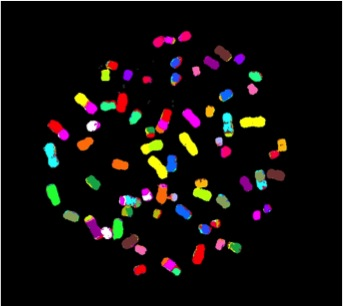
\includegraphics[scale=0.55]{karyograml.jpg}\vspace{-1.29cm}
\caption
{Figure caption. }
\label{fig:f1}
\end{center}
\end{figure*}
%%%%%%%%%%%%%%%%%%%%%%%%%%%%%%%%%%%%%%%%%%%%%%%%

%%%%%%%%%%%%%%%%%%%%%%%%%%%%%%%%%%%%%%%%%%%%%%%%
\begin{figure*}
\begin{center}
% 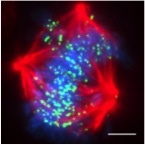
\includegraphics[scale=0.55]{multipolar2l.jpg}
\caption
{Figure caption}
\label{fig:f2}
\end{center}
\end{figure*}
%%%%%%%%%%%%%%%%%%%%%%%%%%%%%%%%%%%%%%%%%%%%%%%%


%-------------------------------------------------%
\section{Section Heading}
%-------------------------------------------------%

Lorem ipsum dolor sit amet, consectetur adipiscing elit. Suspendisse accumsan magna est, quis elementum leo laoreet eu. Donec sollicitudin elit non massa venenatis, in viverra dolor sagittis. Maecenas ac justo pulvinar, consectetur mauris hendrerit, vulputate lacus. Etiam tristique sapien quis sem commodo, et eleifend tortor viverra. In hac habitasse platea dictumst. Phasellus vel tempus risus, sit amet consectetur massa. Duis rutrum lectus eu ligula egestas iaculis. Sed condimentum, ipsum in dignissim condimentum, nisi turpis blandit massa, et aliquam magna ligula eget lacus. Donec ac eleifend nulla, quis cursus nisi. Lorem ipsum dolor sit amet, consectetur adipiscing elit. Suspendisse accumsan magna est, quis elementum leo laoreet eu. Donec sollicitudin elit non massa venenatis, in viverra dolor sagittis. Maecenas ac justo pulvinar, consectetur mauris hendrerit, vulputate lacus. Etiam tristique sapien quis sem commodo, et eleifend tortor viverra. In hac habitasse platea dictumst. Phasellus vel tempus risus, sit amet consectetur massa. Duis rutrum lectus eu ligula egestas iaculis. Sed condimentum, ipsum in dignissim condimentum, nisi turpis blandit massa, et aliquam magna ligula eget lacus. Donec ac eleifend nulla, quis cursus nisi.

Lorem ipsum dolor sit amet, consectetur adipiscing elit. Suspendisse accumsan magna est, quis elementum leo laoreet eu. Donec sollicitudin elit non massa venenatis, in viverra dolor sagittis. Maecenas ac justo pulvinar, consectetur mauris hendrerit, vulputate lacus. Etiam tristique sapien quis sem commodo, et eleifend tortor viverra.

\bibliographystyle{abbrvnat}
\bibliography{winnower_template}

\appendix

\section{Appendix Heading}
Lorem ipsum dolor sit amet, consectetur adipiscing elit. Suspendisse accumsan magna est, quis elementum leo laoreet eu. Donec sollicitudin elit non massa venenatis, in viverra dolor sagittis. Maecenas ac justo pulvinar, consectetur mauris hendrerit, vulputate lacus. Etiam tristique sapien quis sem commodo, et eleifend tortor viverra. In hac habitasse platea dictumst. Phasellus vel tempus risus, sit amet consectetur massa. Duis rutrum lectus eu ligula egestas iaculis. Sed condimentum, ipsum in dignissim condimentum, nisi turpis blandit massa, et aliquam magna ligula eget lacus. Donec ac eleifend nulla, quis cursus nisi. Lorem ipsum dolor sit amet, consectetur adipiscing elit. Suspendisse accumsan magna est, quis elementum leo laoreet eu. Donec sollicitudin elit non massa venenatis, in viverra dolor sagittis. Maecenas ac justo pulvinar, consectetur mauris hendrerit, vulputate lacus. Etiam tristique sapien quis sem commodo, et eleifend tortor viverra. In hac habitasse platea dictumst. Phasellus vel tempus risus, sit amet consectetur massa. Duis rutrum lectus eu ligula egestas iaculis. Sed condimentum, ipsum in dignissim condimentum, nisi turpis blandit massa, et aliquam magna ligula eget lacus. Donec ac eleifend nulla, quis cursus nisi.

\end{document}
